% !TeX spellcheck = en_US
\cleardoublepage\phantomsection\addcontentsline{toc}{section}{\protect\numberline{} {} {} {} {}Dungeons and Devils}
\addscenariosection[subsection]{1}{Inferno Campaign $-$ Dungeons and Devils}{1. A Devilish Plan}{\images/firewall.png}

\begin{multicols*}{2}

\textbf{Author:} Tm335

\textbf{Source:} \href{https://discord.com/channels/740870068178649108/1243057664666238996/1243057664666238996}{Archon Studios Discord}

\textit{A large elvish population inhabits Erathia's southeastern coast.
Green and gold dragons, native to the region, augment their military strength.
Before we conquer this region and redirect our forces to Steadwick, we must annihilate these dragons.
Our Kreegan allies from Eeofol have requested the honor of this mission.
The Kreegans are fierce warriors; they will relish the slaughter.}

\subsection*{\MakeUppercase{Scenario length}}

This scenario plays out over 13 rounds.

\subsection*{\MakeUppercase{Player setup}}

\textbf{Faction:} Inferno

\textbf{Faction Hero:} Choose any

\textbf{Starting Resources:} 15 \svg{gold}, 3 \svg{building_materials}, 1 \svg{valuables}

\textbf{Starting Income:} 10 \svg{gold}, 0 \svg{building_materials}, 0 \svg{valuables}

\textbf{Starting Units:}

\begin{itemize}
  \item A Pack of Familiars
  \item A Few Magogs
\end{itemize}

\textbf{Town Buildings:} \svgunit{bronze} Dwelling, City Hall

\textbf{Bonus:} Choose one of the following options:
\begin{itemize}
  \item Add a ``Slayer'' spell to your hand
  \item Add the ``Armor of Wonder'' Artifact to your hand
  \item Reinforce Magogs and gain 1 \svg{valuables}
\end{itemize}

\subsection*{\MakeUppercase{AI hero setup}}

\textbf{Faction:} Rampart

\textbf{Enemy Armies:}

\begin{itemize}
  \item \textbf{Gold Dragon Army:} A Pack of Gold Dragons, a Pack of Unicorns, a Pack of Dendroids, a Pack of Centaurs
  \item \textbf{Ivor's Army:} A Few Elves\footnote{In Round 9, the Few Elves in Ivor's Army are reinforced to a Pack of Elves.}, Neutral Army at the same level as your Hero level\footnote{See page 35, ``Field Difficulty Level Table'' in the Core Rulebook, for further details on the number of Neutral Units you have to draw for this Neutral Army.}
\end{itemize}

\textbf{Ivor's Deck:} 1 × Might card, 2 × Magic card, 1 × Skill card

\textbf{Ivor's Spell Deck:} 1 × Precision Spell card (it resolves on the first \svg{unit_ranged} unit able to make a \svg{unit_ranged} attack), 1 × Magic Arrow Spell card

\textbf{Ivor's Skill:} Archery Ability card (it always resolves its Basic effect)

\subsection*{\MakeUppercase{Map setup}}

Take the following Map tiles and arrange them as shown in the scenario map layout:

\textbf{2 × Starting (I) Map tile}
\begin{itemize}
  \item 1 × Inferno (S6)
  \item 1 × Rampart (S4)
\end{itemize}

\textbf{3 × Far (II--III) Map tile}
\begin{itemize}
  \item \mbox{2 × Inferno (choose from: F16--F18, \#F10)}
  \item 1 × Rampart (choose from: F10--F12)
\end{itemize}

\textbf{2 × Near (IV--V) Map tile}
\begin{itemize}
  \item 2 × Rampart (N7, N8)
\end{itemize}

\textbf{1 × Center (VI--VII) Map tile}
\begin{itemize}
  \item 1 × Dragon Utopia Center Map tile (C1)
\end{itemize}

\subsection*{\MakeUppercase{Heroes placement}}

The Enemy Hero is represented by one Rampart faction Hero model of your choice
and appears in the center field of the S4 Starting Map tile.

Place your Hero in the center field of the Inferno Starting Map tile.

\subsection*{\MakeUppercase{Victory Conditions}}

Defeat the Enemy Hero and the Gold Dragons Armies.

\subsection*{\MakeUppercase{Defeat Conditions}}

You lose one Combat encounter.

You fail to defeat the Enemy Hero and the Gold Dragon Armies by the end of the Round 13.

\subsection*{\MakeUppercase{Timed Events}}

\textbf{\nth{1} Round:}
\begin{itemize}
  \item Read: ``Our underlings have done well. They have managed to raise a volcano
    and erect a fort in a sparsely populated forest just outside of Erathia's border.
    While the Dungeon Overlords make their way underground toward the Erathian capitol,
    you must strike at their allies, the elves of AvLee.''
\end{itemize}

\textbf{\nth{2} Round:}
\begin{itemize}
  \item Read: ``The Gold Dragon Queen is a powerful ally of AvLee.
    You must find her lair and see to her demise, as this will greatly weaken
    the elves and make them less of a threat to our plans to destroy Erathia.
    Go now, and make us proud!''
\end{itemize}

\textbf{\nth{9} Round:}
\begin{itemize}
  \item The Few Elves of Ivor's Army are Reinforced to a Pack of Elves.
    Ivor's Army also gains an Ammo Cart.
\end{itemize}

\textbf{\nth{10} Round:}
\begin{itemize}
  \item The Rampart Faction Town that Ivor's Army resides in gains an Arrow Tower.
\end{itemize}

\textbf{\nth{13} Round:}
\begin{itemize}
  \item At the end of the round, if both the Enemy Hero and the Gold Dragon Armies are not defeated, all is lost -- you lose!
\end{itemize}

\textbf{When you complete the scenario:}
\begin{itemize}
  \item Read: ``Congratulations! You have completed your quest to kill the fearsome beast, and can claim victory!''
\end{itemize}


\subsection*{\MakeUppercase{Additional rules}}

During this ``Inferno'' campaign scenario, the following rules apply:

\begin{itemize}
    \item Your Hero does not gain Experience past Level 5.
    \item The Enemy Hero does not move and only waits in their Town. They start with Walls and a Gate on their side of the Combat Board.
    \item The N7 Map tile cannot be entered until Ivor is defeated.
    \item At the Dragon Utopia location, your Hero fights the Gold Dragons Army.
    \item The ``Castle Gate'' cannot be built.
    \item If your Hero visits an Obelisk, you may Search (2) the Ability deck, the Artifact deck, or the Spell deck.
\end{itemize}

\vspace*{\fill}
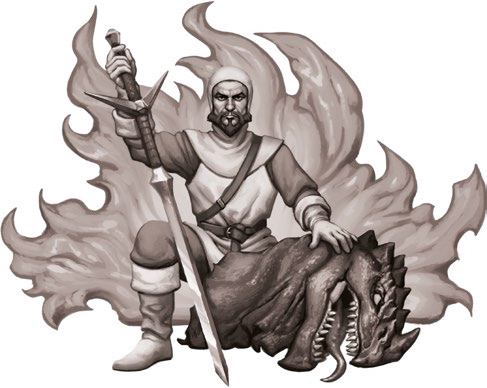
\includegraphics[width=0.4\paperwidth, keepaspectratio]{\art/slayer.png}
\vspace*{\fill}

\end{multicols*}

\begin{tikzpicture}[remember picture, overlay]
  \node(bg)[anchor=center, yshift=37em, opacity=0.5] at (current page.south) {
    
\includegraphics[width=0.85\paperwidth, keepaspectratio]{\art/fire_magic.png}
  };
  \node(map)[anchor=center] at (current page.center) {
    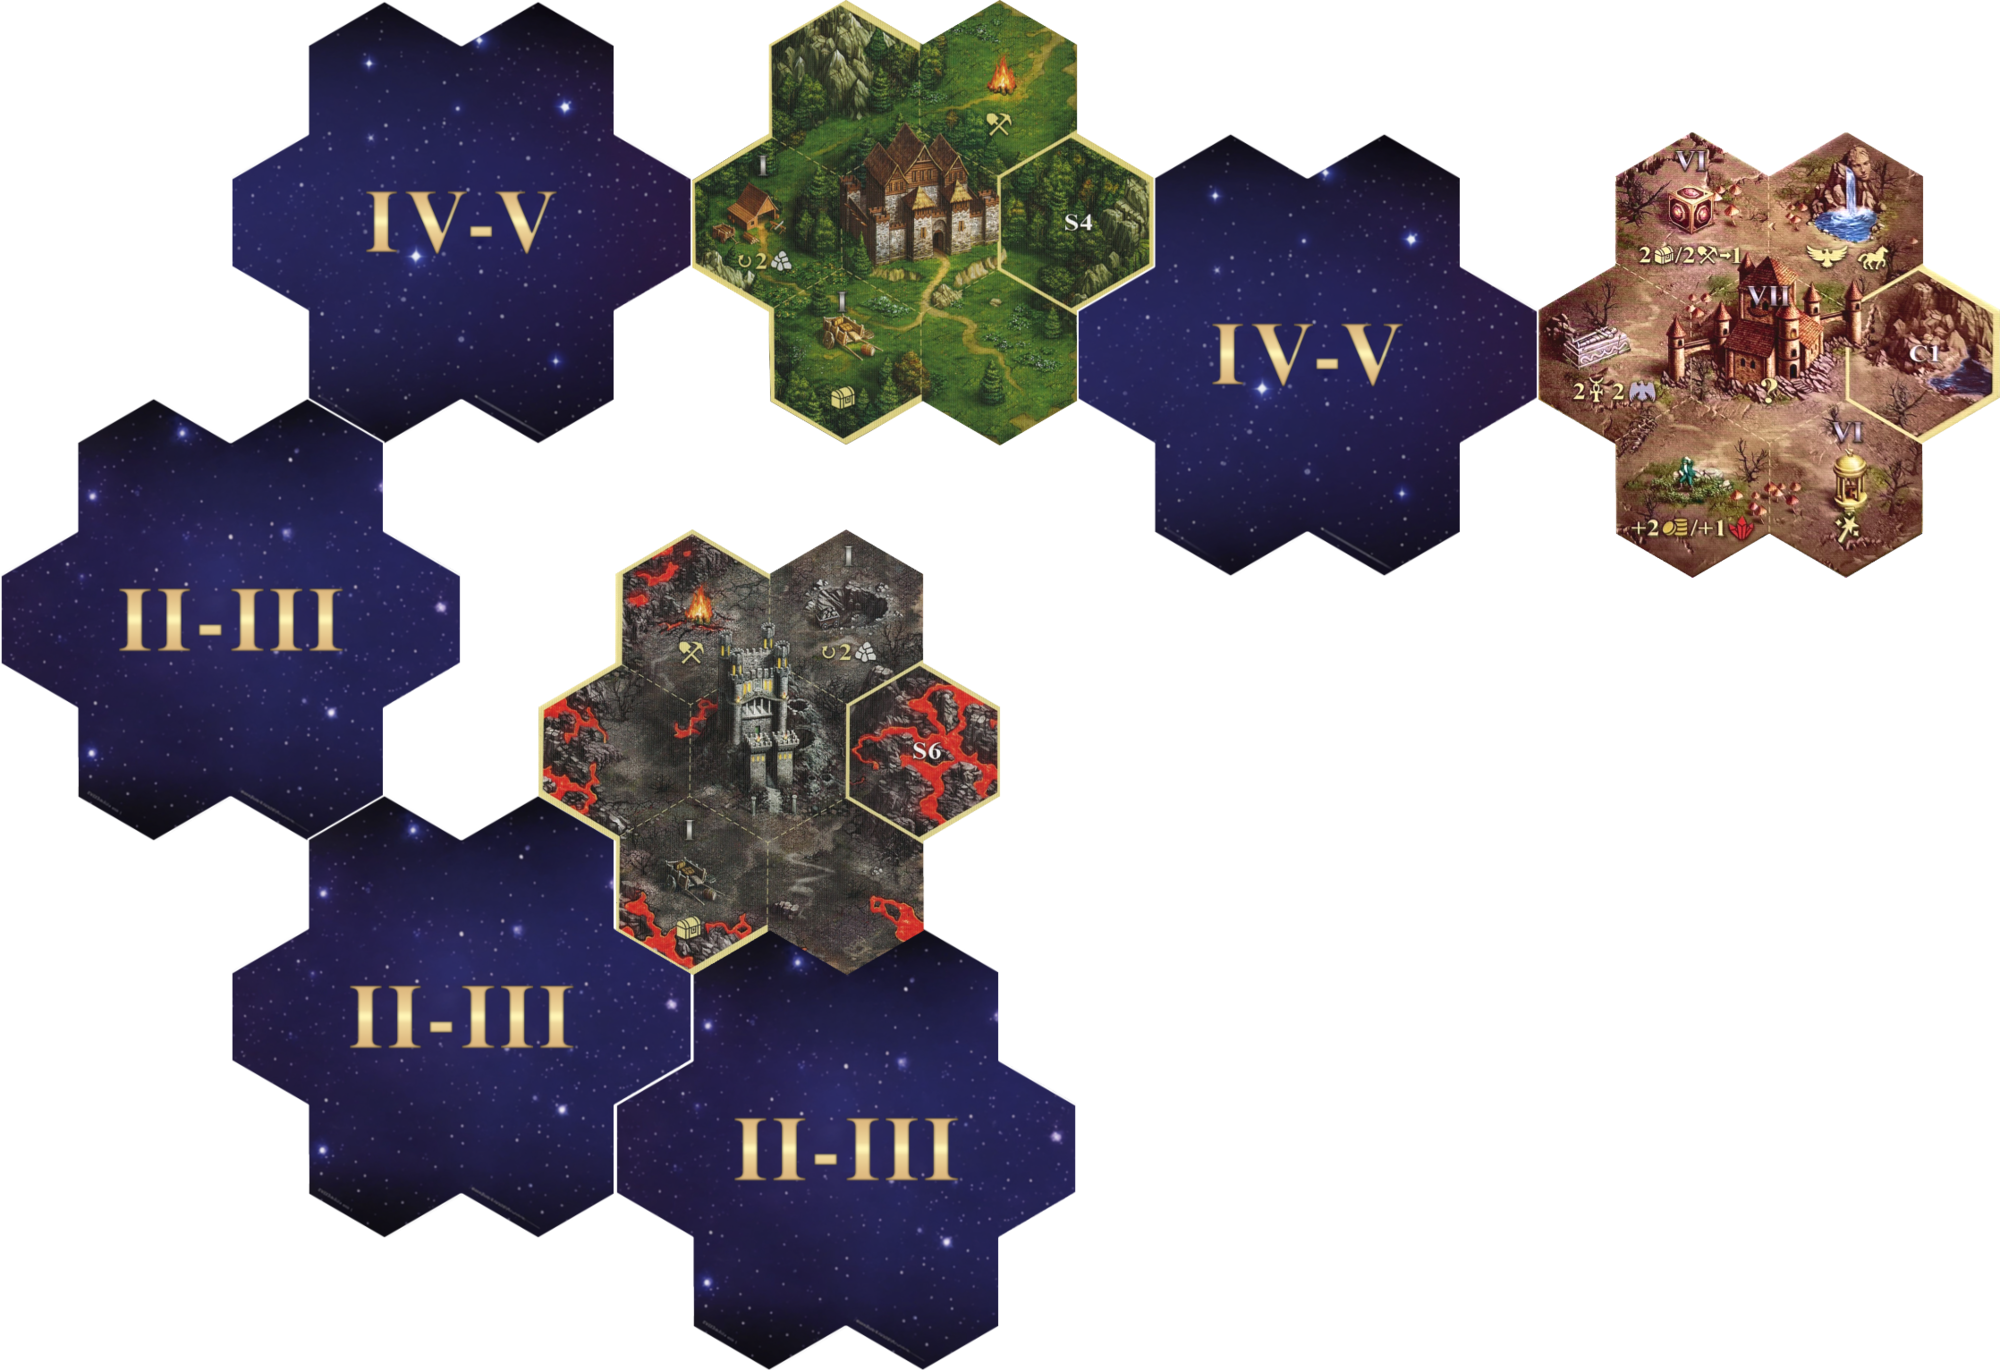
\includegraphics[width=\textwidth]{\maps/inferno_devilish_plan.png}
  };
  \node at (2,-6.5) {\large{{\textbf{\textcolor{darkcandyapplered}{N8}}}}};
  \node at (13, -6.5) {\large{{\textbf{\textcolor{darkcandyapplered}{N7}}}}};
  \node at (4.8, -17.6) {\large{{\textbf{\textcolor{darkcandyapplered}{Inferno}}}}};
  \node at (4.8, -18.3) {\large{{\textbf{\textcolor{darkcandyapplered}{Map Tiles}}}}};
\end{tikzpicture}
